\documentclass[border=8pt]{standalone}
\usepackage{fontspec}\usepackage{tikz}
\usetikzlibrary{arrows.meta,positioning,calc}
\definecolor{NouOrange}{HTML}{FA4D1F}\definecolor{NouBlack}{HTML}{000000}
\begin{document}
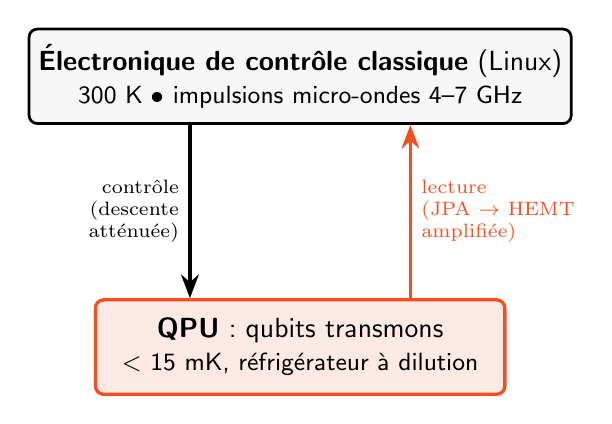
\begin{tikzpicture}[font=\sffamily,
  b/.style={draw=NouBlack,line width=1pt,rounded corners=3pt,align=center,minimum width=5.2cm,minimum height=1.2cm,fill=black!3}]
  \node[b] (ctrl) {\textbf{Électronique de contrôle classique} (Linux)\\{\small 300 K \textbullet{} impulsions micro-ondes 4--7 GHz}};
  \node[b,below=2.2cm of ctrl,fill=NouOrange!12,draw=NouOrange,line width=1.2pt] (qpu) {\textbf{QPU} : qubits transmons\\{\small $<$ 15 mK, réfrigérateur à dilution}};
  \draw[-{Stealth[length=3mm]},NouBlack,line width=1.3pt] ($(ctrl.south)+(-1.4cm,0)$) -- node[left,align=right,font=\scriptsize]{contrôle\\(descente\\atténuée)} ($(qpu.north)+(-1.4cm,0)$);
  \draw[-{Stealth[length=3mm]},NouOrange,line width=1.3pt] ($(qpu.north)+(1.4cm,0)$) -- node[right,align=left,font=\scriptsize]{lecture\\(JPA $\to$ HEMT\\amplifiée)} ($(ctrl.south)+(1.4cm,0)$);
\end{tikzpicture}
\end{document}
